% Appendices are not given names in this style
\section{}
\justify

% Longtable allows tables to span multiple pages. Not possible with tabularx
\begin{longtable}{llll}
    % define longtable header for the first page
    \caption[PAAVO postal code areas]{PAAVO postal code areas in Helsinki Capital Region.} \\
    \label{tab:appendix_postalcodes} \\
    \hline
    Postal code & Name (fi) & Name (sv) & Municipality \\ [0.5ex]
    \hline\hline
    \endfirsthead % all lines above this command will be repeated on every page
    
    % define longtable header for all subsequent pages
    \multicolumn{4}{c}%
        {\textbf{\tablename\ \thetable.} PAAVO postal code areas, continued from previous pages.} \\ [1.25ex]
    \hline
    Postal code & Name (fi) & Name (sv) & Municipality \\ [0.5ex]
    \hline\hline 
    \endhead
    
    % Content proper
    00100 & Helsinki Keskusta - Etu-Töölö & Helsingfors centrum - Främre Tölö & Helsinki \\ [0.5 ex] \hline
    00120 & Punavuori & Rödbergen & Helsinki \\ [0.25ex] \hline
    00130 & Kaartinkaupunki & Gardesstaden & Helsinki \\ [0.25ex] \hline
    00140 & Kaivopuisto - Ullanlinna & Brunnsparken - Ulrikasborg & Helsinki \\ [0.25ex] \hline
    00150 & Eira - Hernesaari & Eira - Ärtholmen & Helsinki \\ [0.25ex] \hline
    00160 & Katajanokka & Skatudden & Helsinki \\ [0.25ex] \hline
    00170 & Kruununhaka & Kronohagen & Helsinki \\ [0.25ex] \hline
    00180 & Kamppi - Ruoholahti & Kampen - Gräsviken & Helsinki  \\ [0.25ex] \hline
    00190 & Suomenlinna & Sveaborg & Helsinki \\ [0.25ex] \hline
    00200 & Lauttasaari & Drumsö & Helsinki \\ [0.25ex] \hline
    00210 & Vattuniemi & Hallonnäs & Helsinki \\ [0.25ex] \hline
    00220 & Jätkäsaari & Busholmen & Helsinki \\ [0.25ex] \hline
    00230 & Ilmala & Ilmala & Helsinki \\ [0.25ex] \hline
    00240 & Länsi-Pasila & Västra Böle & Helsinki \\ [0.25ex] \hline
    00250 & Taka-Töölö & Bortre Tölö & Helsinki \\ [0.25ex] \hline
    00260 & Keski-Töölö & Mellersta Tölö & Helsinki \\ [0.25ex] \hline
    00270 & Pohjois-Meilahti & Norra Mejlans & Helsinki \\ [0.25ex] \hline
    00280 & Ruskeasuo & Brunakärr & Helsinki \\ [0.25ex] \hline
    00290 & Meilahden sairaala-alue & Mejlans sjukhusområde & Helsinki \\ [0.25ex] \hline
    00300 & Pikku Huopalahti & Lillhoplax & Helsinki \\ [0.25ex] \hline
    00310 & Kivihaka & Stenhagen & Helsinki \\ [0.25ex] \hline
    00320 & Etelä-Haaga & Södra Haga & Helsinki \\ [0.25ex] \hline
    00330 & Munkkiniemi & Munksnäs & Helsinki \\ [0.25ex] \hline
    00340 & Kuusisaari-Lehtisaari & Granö-Lövö & Helsinki \\ [0.25ex] \hline
    00350 & Munkkivuori-Niemenmäki & Munkshöjden-Näshöjden & Helsinki\\ [0.25ex] \hline
    00360 & Pajamäki & Smedjebacka & Helsinki \\ [0.25ex] \hline
    00370 & Reimarla & Reimars & Helsinki \\ [0.25ex] \hline
    00380 & Pitäjänmäen teollisuusalue & Sockenbacka industriområde & Helsinki \\ [0.25ex] \hline
    00390 & Konala & Kånala & Helsinki \\ [0.25ex] \hline
    00400 & Pohjois-Haaga & Norra Haga & Helsinki \\ [0.25ex] \hline
    00410 & Malminkartano & Malmgård & Helsinki \\ [0.25ex] \hline
    00420 & Kannelmäki & Gamlas & Helsinki \\ [0.25ex] \hline
    00430 & Maununneva & Magnuskärr & Helsinki \\ [0.25ex] \hline
    00440 & Lassila & Lassas & Helsinki \\ [0.25ex] \hline
    00500 & Sörnäinen & Sörnäs & Helsinki \\ [0.25ex] \hline
    00510 & Etu-Vallila - Alppila & Främre Vallgård - Alphyddan & Helsinki \\ [0.25ex] \hline
    00520 & Itä-Pasila & Östra Böle & Helsinki \\ [0.25ex] \hline
    00530 & Kallio & Berghäll & Helsinki \\ [0.25ex] \hline
    00540 & Kalasatama & Fiskhamnen & Helsinki \\ [0.25ex] \hline
    00550 & Vallila & Vallgård & Helsinki \\ [0.25ex] \hline
    00560 & Toukola-Vanhakaupunki & Majstad-Gammelstad & Helsinki \\ [0.25ex] \hline
    00570 & Kulosaari & Brändö & Helsinki \\ [0.25ex] \hline
    00580 & Verkkosaari & Nätholmen & Helsinki \\ [0.25ex] \hline
    00590 & Kaitalahti & Hålvik & Helsinki \\ [0.25ex] \hline
    00600 & Koskela-Helsinki & Forsby-Helsingfors & Helsinki \\ [0.25ex] \hline
    00610 & Käpylä & Kottby & Helsinki \\ [0.25ex] \hline
    00620 & Metsälä-Etelä-Oulunkylä & Krämertsskog-Södra Åggelby & Helsinki \\ [0.25ex] \hline
    00630 & Maunula-Suursuo & Månsas-Storkärr & Helsinki \\ [0.25ex] \hline
    00640 & Oulunkylä-Patola & Åggelby-Dammen & Helsinki \\ [0.25ex] \hline
    00650 & Veräjämäki & Grindbacka & Helsinki \\ [0.25ex] \hline
    00660 & Länsi-Pakila & Västra Baggböle & Helsinki \\ [0.25ex] \hline
    00670 & Paloheinä & Svedängen & Helsinki \\ [0.25ex] \hline
    00680 & Itä-Pakila & Östra Baggböle & Helsinki \\ [0.25ex] \hline
    00690 & Tuomarinkylä-Torpparinmäki & Domarby-Torparbacken & Helsinki \\ [0.25ex] \hline
    00700 & Malmi & Malm & Helsinki \\ [0.25ex] \hline
    00710 & Pihlajamäki & Rönnbacka & Helsinki \\ [0.25ex] \hline
    00720 & Pukinmäki-Savela & Bocksbacka-Lerstrand & Helsinki \\ [0.25ex] \hline
    00730 & Tapanila & Mosabacka & Helsinki \\ [0.25ex] \hline
    00740 & Siltamäki & Brobacka & Helsinki \\ [0.25ex] \hline
    00750 & Puistola & Parkstad & Helsinki \\ [0.25ex] \hline
    00760 & Suurmetsä & Storskog & Helsinki \\ [0.25ex] \hline
    00770 & Jakomäki - Alppikylä & Jakobacka - Alpbyn & Helsinki \\ [0.25ex] \hline
    00780 & Tapaninvainio & Staffansslätten & Helsinki \\ [0.25ex] \hline
    00790 & Viikki & Vik & Helsinki \\ [0.25ex] \hline
    00800 & Länsi-Herttoniemi & Västra Hertonäs & Helsinki \\ [0.25ex] \hline
    00810 & Herttoniemi & Hertonäs & Helsinki \\ [0.25ex] \hline
    00820 & Roihuvuori & Kasberget & Helsinki \\ [0.25ex] \hline
    00830 & Tammisalo & Tammelund & Helsinki \\ [0.25ex] \hline
    00840 & Laajasalo & Degerö & Helsinki \\ [0.25ex] \hline
    00850 & Jollas & Jollas & Helsinki \\ [0.25ex] \hline
    00860 & Santahamina & Sandhamn & Helsinki \\ [0.25ex] \hline
    00870 & Etelä-Laajasalo & Södra Degerö & Helsinki \\ [0.25ex] \hline
    00880 & Roihupellon teollisuusalue & Kasåkerns industriområde & Helsinki \\ [0.25ex] \hline
    00890 & Itäsalmi & Östersundom & Helsinki \\ [0.25ex] \hline
    00900 & Puotinharju & Botbyhöjden & Helsinki \\ [0.25ex] \hline
    00910 & Puotila & Botby gård & Helsinki \\ [0.25ex] \hline
    00920 & Myllypuro & Kvarnbäcken & Helsinki \\ [0.25ex] \hline
    00930 & Itäkeskus-Marjaniemi & Östra centrum-Marudd & Helsinki \\ [0.25ex] \hline
    00940 & Kontula - Vesala & Gårdsbacka - Ärvings & Helsinki \\ [0.25ex] \hline
    00950 & Vartioharju & Botbyåsen & Helsinki \\ [0.25ex] \hline
    00960 & Pohjois-Vuosaari & Norra  Nordsjö & Helsinki \\ [0.25ex] \hline
    00970 & Mellunmäki & Mellungsbacka & Helsinki \\ [0.25ex] \hline
    00980 & Etelä-Vuosaari & Södra Nordsjö & Helsinki \\ [0.25ex] \hline
    00990 & Aurinkolahti & Solvik & Helsinki \\ [0.25ex] \hline
    01200 & Hakunila & Håkansböle & Vantaa \\ [0.25ex] \hline
    01230 & Vaarala & Fagersta & Vantaa \\ [0.25ex] \hline
    01260 & Itä-Hakkila & Östra Haxböle & Vantaa \\ [0.25ex] \hline
    01280 & Länsimäki & Västerkulla & Vantaa \\ [0.25ex] \hline
    01300 & Tikkurila & Dickursby & Vantaa \\ [0.25ex] \hline
    01340 & Leinelä & Lejle & Vantaa \\ [0.25ex] \hline
    01350 & Hiekkaharju & Sandkulla & Vantaa \\ [0.25ex] \hline
    01360 & Koivukylä-Havukoski & Björkby-Havukoski & Vantaa \\ [0.25ex] \hline
    01370 & Jokiniemi & Ånäs & Vantaa \\ [0.25ex] \hline
    01380 & Kuusikko-Hakkila & Sexan-Håkansböle & Vantaa \\ [0.25ex] \hline
    01390 & Ruskeasanta-Ilola & Rödsand-Gladas & Vantaa \\ [0.25ex] \hline
    01400 & Rekola & Räckhals & Vantaa \\ [0.25ex] \hline
    01420 & Päiväkumpu & Lövkulla & Vantaa \\ [0.25ex] \hline
    01450 & Korso & Korso & Vantaa \\ [0.25ex] \hline
    01480 & Mikkola & Mikkola & Vantaa \\ [0.25ex] \hline
    01510 & Kirkonkylä-Veromäki & Kyrkoby-Skattbacka & Vantaa \\ [0.25ex] \hline
    01520 & Tammisto & Rosendal & Vantaa \\ [0.25ex] \hline
    01530 & Veromiehenkylä & Skattmansby & Vantaa \\ [0.25ex] \hline
    01600 & Myyrmäki & Myrbacka & Vantaa \\ [0.25ex] \hline
    01610 & Kaivoksela & Gruvsta & Vantaa \\ [0.25ex] \hline
    01620 & Martinlaakso & Mårtensdal & Vantaa \\ [0.25ex] \hline
    01630 & Hämeenkylä & Tavastby & Vantaa \\ [0.25ex] \hline
    01640 & Hämevaara & Tavastberga & Vantaa \\ [0.25ex] \hline
    01650 & Vapaala & Friherrs & Vantaa \\ [0.25ex] \hline
    01660 & Varisto & Varistorna & Vantaa \\ [0.25ex] \hline
    01670 & Vantaanlaakso & Vandadalen & Vantaa \\ [0.25ex] \hline
    01680 & Askisto & Askis & Vantaa \\ [0.25ex] \hline
    01690 & Ylästö & Övitsböle & Vantaa \\ [0.25ex] \hline
    01700 & Kivistö & Kivistö & Vantaa \\ [0.25ex] \hline
    01710 & Pähkinärinne & Hasselbacken & Vantaa \\ [0.25ex] \hline
    01720 & Petikko & Petikko & Vantaa \\ [0.25ex] \hline
    01730 & Vantaanpuisto & Vandaparken & Vantaa \\ [0.25ex] \hline
    01740 & Tuupakan teollisuusalue & Stubbacka industriområde & Vantaa \\ [0.25ex] \hline
    01750 & Keimola & Käinby & Vantaa \\ [0.25ex] \hline
    01760 & Seutula & Sjöskog & Vantaa \\ [0.25ex] \hline
    01770 & Martinlaakson teollisuusalue & Mårtensdals industriområde & Vantaa \\ [0.25ex] \hline
    02100 & Tapiola & Hagalund & Espoo \\ [0.25ex] \hline
    02110 & Otsolahti & Björnviken & Espoo \\ [0.25ex] \hline
    02120 & Länsikorkee-Suvikumpu & Västerhöjden-Solhöjden & Espoo \\ [0.25ex] \hline
    02130 & Pohjois-Tapiola & Norra Hagalund & Espoo \\ [0.25ex] \hline
    02140 & Laajalahti & Bredvik & Espoo \\ [0.25ex] \hline
    02150 & Otaniemi & Otnäs & Espoo \\ [0.25ex] \hline
    02160 & Westend & Westend & Espoo \\ [0.25ex] \hline
    02170 & Haukilahti & Gäddvik & Espoo \\ [0.25ex] \hline
    02180 & Mankkaa & Mankans & Espoo \\ [0.25ex] \hline
    02200 & Niittykumpu & Ängskulla & Espoo \\ [0.25ex] \hline
    02210 & Olari & Olars & Espoo \\ [0.25ex] \hline
    02230 & Matinkylä & Mattby & Espoo \\ [0.25ex] \hline
    02240 & Friisilä & Frisans & Espoo \\ [0.25ex] \hline
    02250 & Henttaa & Hemtans & Espoo \\ [0.25ex] \hline
    02260 & Kaitaa & Kaitans & Espoo \\ [0.25ex] \hline
    02270 & Finnoo-Eestinmalmi & Finno-Estmalmen & Espoo \\ [0.25ex] \hline
    02280 & Malminmäki-Eestinlaakso & Malmbacka-Estdalen & Espoo \\ [0.25ex] \hline
    02290 & Puolarmetsän sairaala & Bolarskogs sjukhus & Espoo \\ [0.25ex] \hline
    02300 & Nöykkiönpuro & Nöykisbäcken & Espoo \\ [0.25ex] \hline
    02320 & Espoonlahti & Esboviken & Espoo \\ [0.25ex] \hline
    02330 & Saunalahti-Kattilalaakso & Bastvik-Kitteldalen & Espoo \\ [0.25ex] \hline
    02340 & Latokaski & Ladusved & Espoo \\ [0.25ex] \hline
    02360 & Soukka & Sökö & Espoo \\ [0.25ex] \hline
    02380 & Suvisaaristo & Sommaröarna & Espoo \\ [0.25ex] \hline
    02600 & Etelä-Leppävaara & Södra Alberga & Espoo \\ [0.25ex] \hline
    02610 & Kilo & Kilo & Espoo \\ [0.25ex] \hline
    02620 & Karakallio & Karabacka & Espoo \\ [0.25ex] \hline
    02630 & Nihtisilta & Knektbro & Espoo \\ [0.25ex] \hline
    02650 & Pohjois-Leppävaara & Norra Alberga & Espoo \\ [0.25ex] \hline
    02660 & Lintuvaara & Fågelberga & Espoo \\ [0.25ex] \hline
    02680 & Uusmäki & Nybacka & Espoo \\ [0.25ex] \hline
    02700 & Kauniainen & Grankulla & Kauniainen \\ [0.25ex] \hline
    02710 & Viherlaakso & Gröndal & Espoo \\ [0.25ex] \hline
    02720 & Lähderanta & Källstrand & Espoo \\ [0.25ex] \hline
    02730 & Jupperi & Jupper & Espoo \\ [0.25ex] \hline
    02740 & Bemböle-Pakankylä & Bemböle-Backby & Espoo \\ [0.25ex] \hline
    02750 & Sepänkylä-Kuurinniitty & Smedsby-Kurängen & Espoo \\ [0.25ex] \hline
    02760 & Tuomarila-Suvela & Domsby-Södrik & Espoo \\ [0.25ex] \hline
    02770 & Espoon Keskus & Esbo centrum & Espoo \\ [0.25ex] \hline
    02780 & Kauklahti & Köklax & Espoo \\ [0.25ex] \hline
    02810 & Gumböle-Karhusuo & Gumböle-Björnkärr & Espoo \\ [0.25ex] \hline
    02820 & Nupuri-Nuuksio & Nupurböle-Noux & Espoo \\ [0.25ex] \hline
    02860 & Siikajärvi & Siikajärvi & Espoo \\ [0.25ex] \hline
    02920 & Niipperi & Nipert & Espoo \\ [0.25ex] \hline
    02940 & Lippajärvi-Järvenperä & Klappträsk-Träskända & Espoo \\ [0.25ex] \hline
    02970 & Kalajärvi & Kalajärvi & Espoo \\ [0.25ex] \hline
    02980 & Lakisto & Lakisto & Espoo \\ [0.75ex] \hline
\end{longtable}

% \invisiblesection{} is defined to provide a appendix section to the table of contents but not print anything over the appendix II, which is the large postal code area map
\invisiblesection{}
\newgeometry{left=2cm, right=1cm, top=1.75cm, bottom=1.75cm}
\begin{sidewaysfigure}
    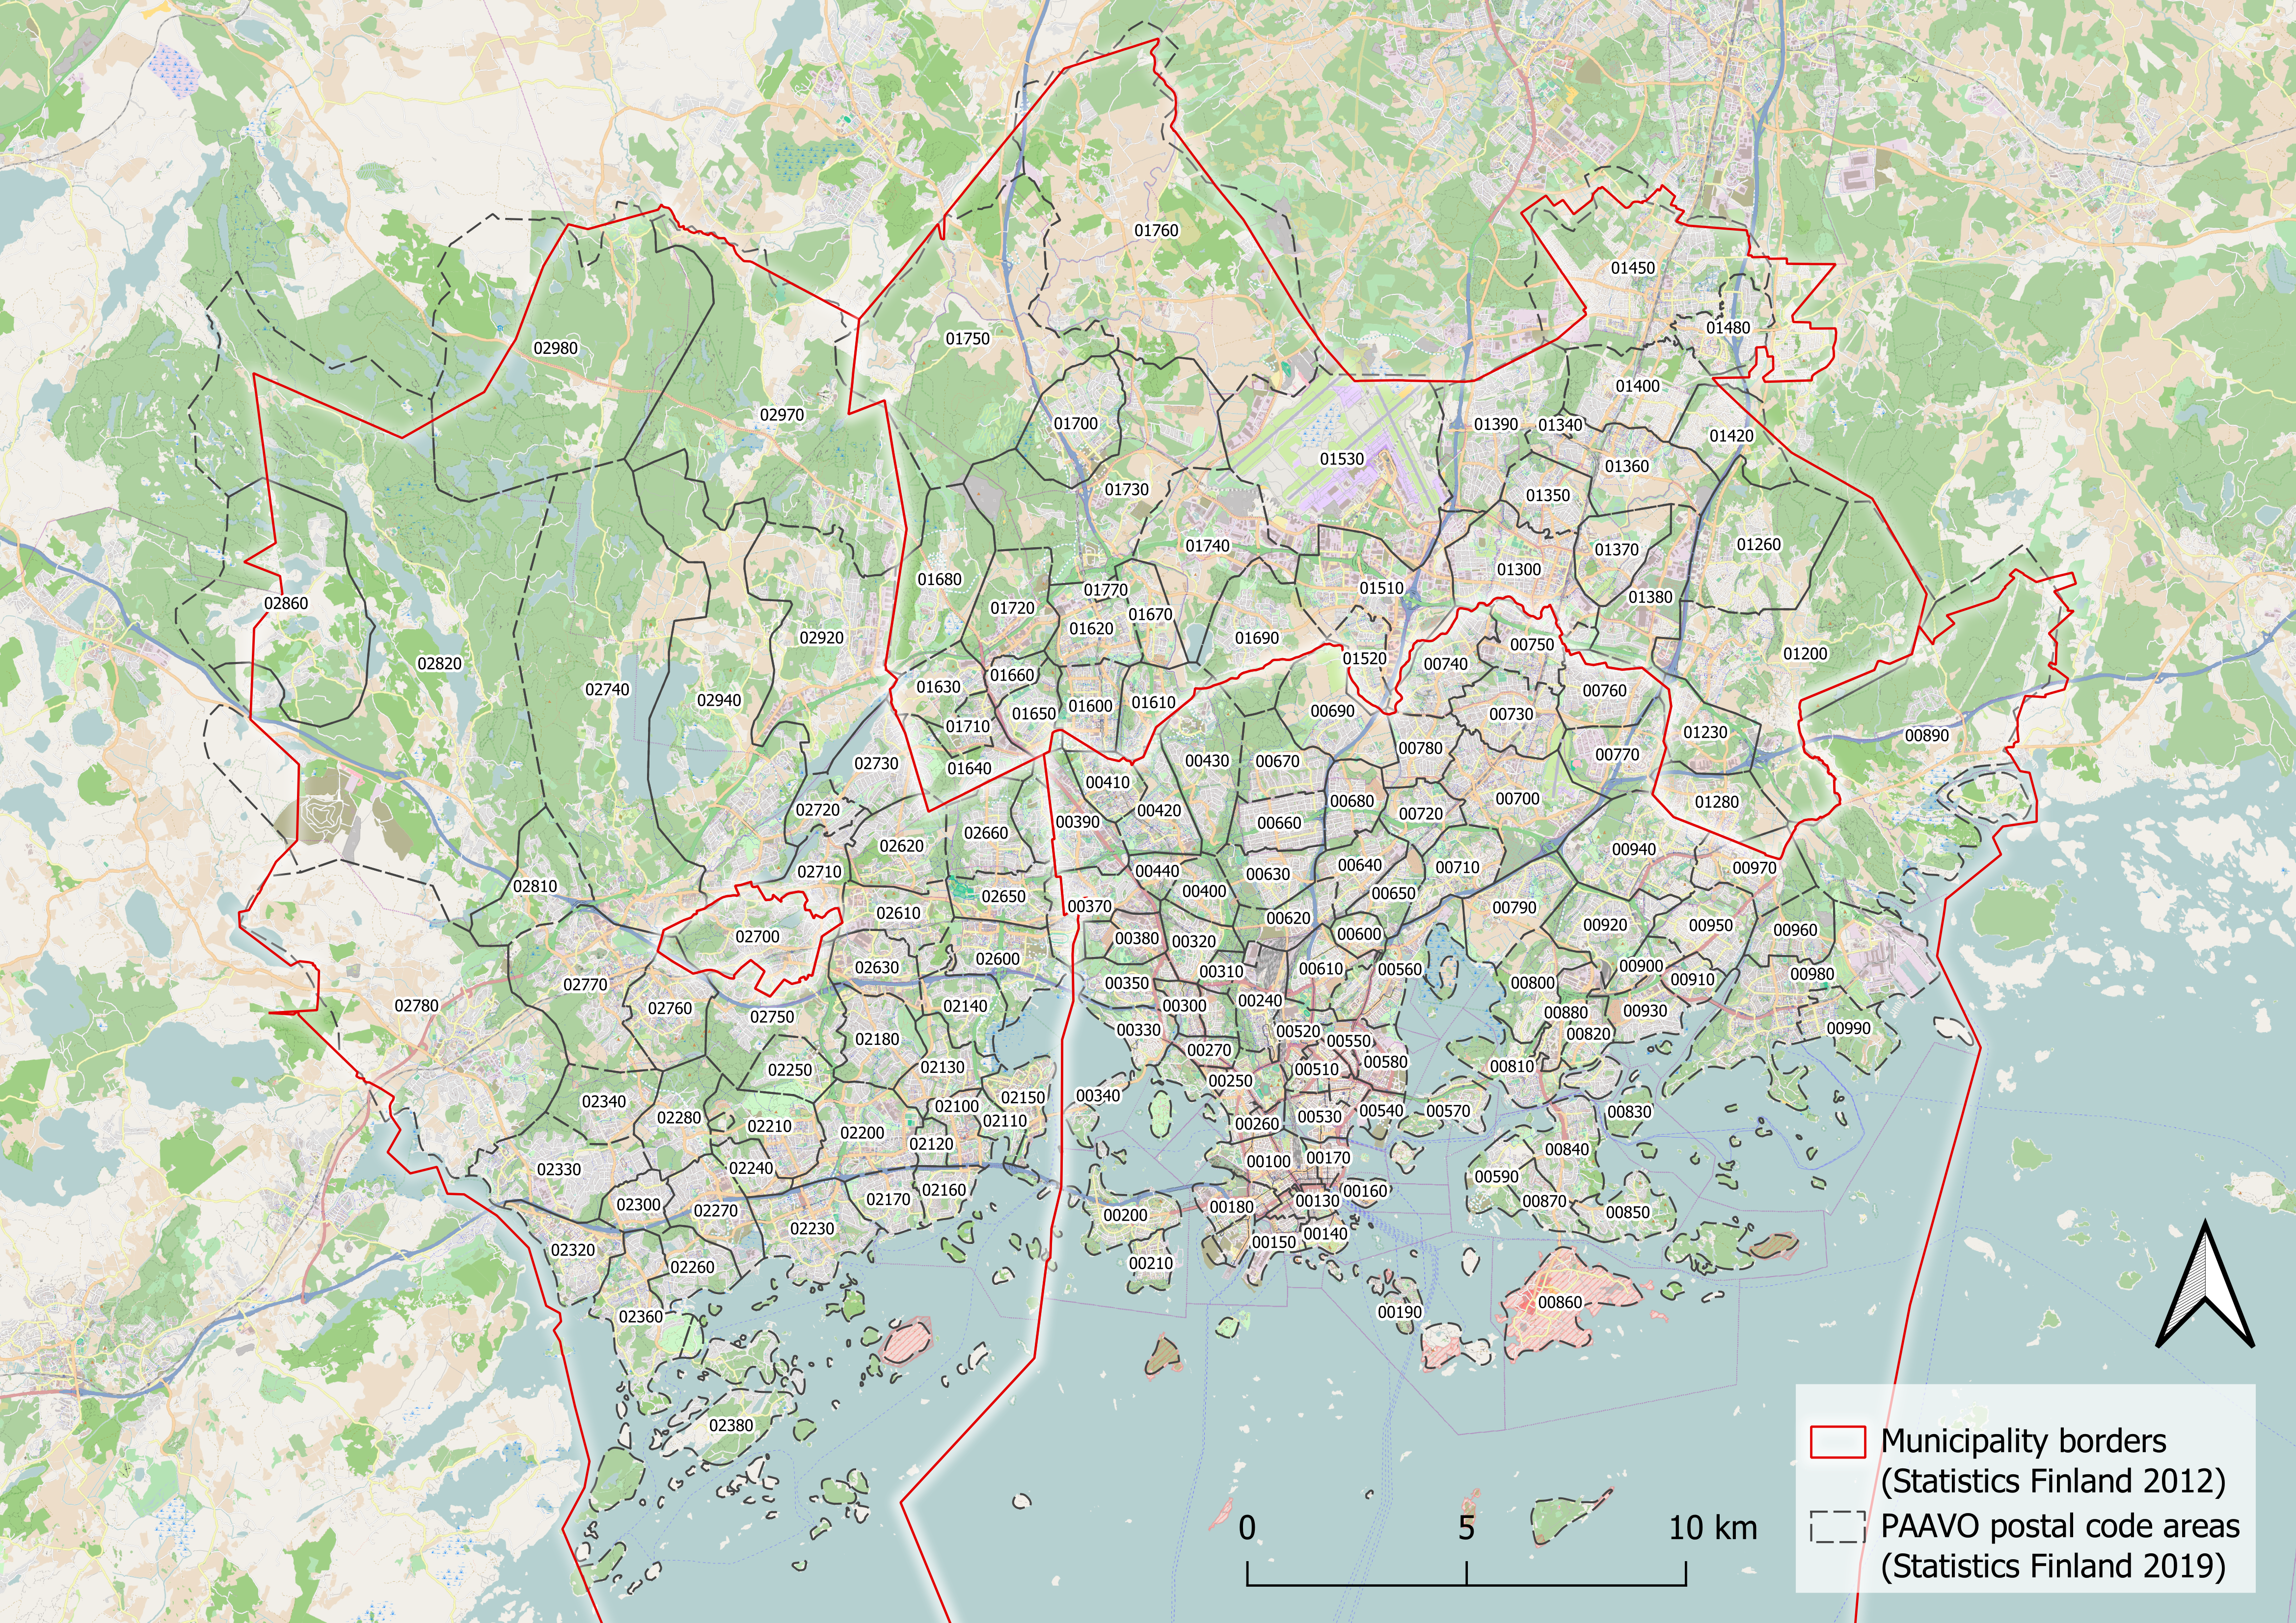
\includegraphics[width=\textwidth]{images/muns_postal_comparison.png}
    \caption[PAAVO postal code areas in the Helsinki Capital Region]{PAAVO postal code areas in the Helsinki Capital Region (\cite{OpenStreetMap}).}
    \label{fig:appendix_muns_postal}
\end{sidewaysfigure}
\restoregeometry

% Rotate content sideways
\newgeometry{left=2cm, right=1cm, top=2cm, bottom=2cm}

% 00520 Itä-Pasila
\begin{sidewaysfigure}
    \section{}
    \centering
    \includegraphics[trim={0.9cm 0.3cm 0.25cm 0.3cm},clip,width=\textwidth]{images/compare_traveltimes_mapfill-msc_r_pct_fromzip-00520_11-10-2020.png}
    \caption[Parking process proportion from Itä-Pasila, rush hour traffic]{The parking process proportion in the total travel chain, in rush hour traffic, starting from 00520 Itä-Pasila. SFP stands for \textit{searching for parking}, \code{parktime}, and WTD \textit{walking to destination}, \code{walktime}. These are the components of the parking process in the \textit{door-to-door approach}.}%
    \label{fig:compare_msc_r_pct_00520}%
\end{sidewaysfigure}

\begin{sidewaysfigure}
    \section{}
    \centering
    \includegraphics[trim={0.9cm 0.3cm 0.25cm 0.3cm},clip,width=\textwidth]{images/compare_traveltimes_mapfill-msc_m_pct_fromzip-00520_11-10-2020.png}
    \caption[Parking process proportion from Itä-Pasila, midday traffic]{The parking process proportion in the total travel chain, in midday traffic, starting from 00520 Itä-Pasila.}%
    \label{fig:compare_msc_m_pct_00520}%
\end{sidewaysfigure}

\begin{sidewaysfigure}
    \section{}
    \centering
    \includegraphics[trim={0.9cm 0.3cm 0.25cm 0.3cm},clip,width=\textwidth]{images/compare_traveltimes_mapfill-msc_all_pct_fromzip-00520_11-10-2020.png}
    \caption[Parking process proportion from Itä-Pasila, all temporal values]{The parking process proportion in the total travel chain, using all temporal values, starting from 00520 Itä-Pasila.}%
    \label{fig:compare_msc_all_pct_00520}%
\end{sidewaysfigure}

% 02650 Pohjois-Leppävaara
\begin{sidewaysfigure}
    \section{}
    \centering
    \includegraphics[trim={0.9cm 0.3cm 0.25cm 0.3cm},clip,width=\textwidth]{images/compare_traveltimes_mapfill-msc_r_pct_fromzip-02650_11-10-2020.png}
    \caption[Parking process proportion from Pohjois-Leppävaara, rush hour traffic]{The parking process proportion in the total travel chain, in rush hour traffic, starting from 02650 Pohjois-Leppävaara. SFP stands for \textit{searching for parking}, \code{parktime}, and WTD \textit{walking to destination}, \code{walktime}. These are the components of the parking process in the \textit{door-to-door approach}.}%
    \label{fig:compare_msc_r_pct_02650}%
\end{sidewaysfigure}

\begin{sidewaysfigure}
    \section{}
    \centering
    \includegraphics[trim={0.9cm 0.3cm 0.25cm 0.3cm},clip,width=\textwidth]{images/compare_traveltimes_mapfill-msc_m_pct_fromzip-02650_11-10-2020.png}
    \caption[Parking process proportion from Pohjois-Leppävaara, midday traffic]{The parking process proportion in the total travel chain, in midday traffic, starting from 02650 Pohjois-Leppävaara.}%
    \label{fig:compare_msc_m_pct_02650}%
\end{sidewaysfigure}

\begin{sidewaysfigure}
    \section{}
    \centering
    \includegraphics[trim={0.9cm 0.3cm 0.25cm 0.3cm},clip,width=\textwidth]{images/compare_traveltimes_mapfill-msc_all_pct_fromzip-02650_11-10-2020.png}
    \caption[Parking process proportion from Pohjois-Leppävaara, all temporal values]{The parking process proportion in the total travel chain, using all temporal values, starting from 02650 Pohjois-Leppävaara.}%
    \label{fig:compare_msc_all_pct_02650}%
\end{sidewaysfigure}

% 00430 Maununneva
\begin{sidewaysfigure}
    \section{}
    \centering
    \includegraphics[trim={0.9cm 0.3cm 0.25cm 0.3cm},clip,width=\textwidth]{images/compare_traveltimes_mapfill-msc_r_pct_fromzip-00430_11-10-2020.png}
    \caption[Parking process proportion from Maununneva, rush hour traffic]{The parking process proportion in the total travel chain, in rush hour traffic, starting from 00430 Maununneva. SFP stands for \textit{searching for parking}, \code{parktime}, and WTD \textit{walking to destination}, \code{walktime}. These are the components of the parking process in the \textit{door-to-door approach}.}%
    \label{fig:compare_msc_r_pct_00430}%
\end{sidewaysfigure}

\begin{sidewaysfigure}
    \section{}
    \centering
    \includegraphics[trim={0.9cm 0.3cm 0.25cm 0.3cm},clip,width=\textwidth]{images/compare_traveltimes_mapfill-msc_m_pct_fromzip-00430_11-10-2020.png}
    \caption[Parking process proportion from Maununneva, midday traffic]{The parking process proportion in the total travel chain, in midday traffic, starting from 00430 Maununneva.}%
    \label{fig:compare_msc_m_pct_00430}%
\end{sidewaysfigure}

\begin{sidewaysfigure}
    \section{}
    \centering
    \includegraphics[trim={0.9cm 0.3cm 0.25cm 0.3cm},clip,width=\textwidth]{images/compare_traveltimes_mapfill-msc_all_pct_fromzip-00430_11-10-2020.png}
    \caption[Parking process proportion from Maununneva, all temporal values]{The parking process proportion in the total travel chain, using all temporal values, starting from 00430 Maununneva.}%
    \label{fig:compare_msc_all_pct_00430}%
\end{sidewaysfigure}

% 01690 Ylästö
\begin{sidewaysfigure}
    \section{}
    \centering
    \includegraphics[trim={0.9cm 0.3cm 0.25cm 0.3cm},clip,width=\textwidth]{images/compare_traveltimes_mapfill-msc_r_pct_fromzip-01690_11-10-2020.png}
    \caption[Parking process proportion from Ylästö, rush hour traffic]{The parking process proportion in the total travel chain, in rush hour traffic, starting from 01690 Ylästö. SFP stands for \textit{searching for parking}, \code{parktime}, and WTD \textit{walking to destination}, \code{walktime}. These are the components of the parking process in the \textit{door-to-door approach}.}%
    \label{fig:compare_msc_r_pct_01690}%
\end{sidewaysfigure}

\begin{sidewaysfigure}
    \section{}
    \centering
    \includegraphics[trim={0.9cm 0.3cm 0.25cm 0.3cm},clip,width=\textwidth]{images/compare_traveltimes_mapfill-msc_m_pct_fromzip-01690_11-10-2020.png}
    \caption[Parking process proportion from Ylästö, midday traffic]{The parking process proportion in the total travel chain, in midday traffic, starting from 01690 Ylästö.}%
    \label{fig:compare_msc_m_pct_01690}%
\end{sidewaysfigure}

\begin{sidewaysfigure}
    \section{}
    \centering
    \includegraphics[trim={0.9cm 0.3cm 0.25cm 0.3cm},clip,width=\textwidth]{images/compare_traveltimes_mapfill-msc_all_pct_fromzip-01690_11-10-2020.png}
    \caption[Parking process proportion from Ylästö, all temporal values]{The parking process proportion in the total travel chain, using all temporal values, starting from 01690 Ylästö.}%
    \label{fig:compare_msc_all_pct_01690}%
\end{sidewaysfigure}
\restoregeometry